\section{Configurazione dell'applicativo progettato e strumenti di sviluppo}

\subsection{Test d'unit\`a}
\label{Test d'unita}
Per eseguire, con successo, i test d'unità è necessario procedere all'installazione, se non gi\`a presenti, dei moduli node\_js e delle componenti aggiuntive necessarie ad una corretta esecuzione degli script. Di seguito riporto le istruzioni per poter effettuare con successo la build dei test implementati \footnote{Se al esecuzione del comando da shall npm test viene generato un errore, seguire i seguenti passi di installazione}.\\
Prima di tutto l'utente deve aprire una \textit{shell da terminale} e spostarsi all'interno delle sottocartelle rete\_neurale/rete neurale nella repository "AI-Reticolo\_della\_conoscenza".
Per poter eseguire i test d'unit\`a su qualsiasi sistema operativo, \`e necessarie procedere alle seguenti installazioni:
\begin{enumerate}
 \item Installare node js da \url{https://nodejs.org/en/download/} per poter usare il comando npm;
 \item Installare mocha: \textbf{npm install mocha};
 \item Installare  il modulo babel core/register: \textbf{npm install --save-dev babel-core babel-preset -env};
 \item Installare presets per 2015:  \textbf{npm install babel-cli babel-preset-es2015};
 \item Installare il modulo chai: \textbf{npm install chai}.
\end{enumerate}
\noindent
Per mandare in esecuzione i test digitare da terminale il comando \textbf{npm test}.\\
Javascript \`e un linguaggio lato client, da browser. I test automatici sono stati sviluppati trasformando le singole unit\`a in moduli node esportati. La sintassi exports poco si adatta all'utilizzo dei browser\footnote{Il supporto viene offerto da Safari 10.1, Chrome 61, Firefox 54, Edge 16} per questo ho deciso di omettere le keywords exports come preambolo dei metodi soggetti a test; tale aggiunta \`e di competenza dell'utente nel momento precedente al test running.

\begin{figure}[H]
\centering
	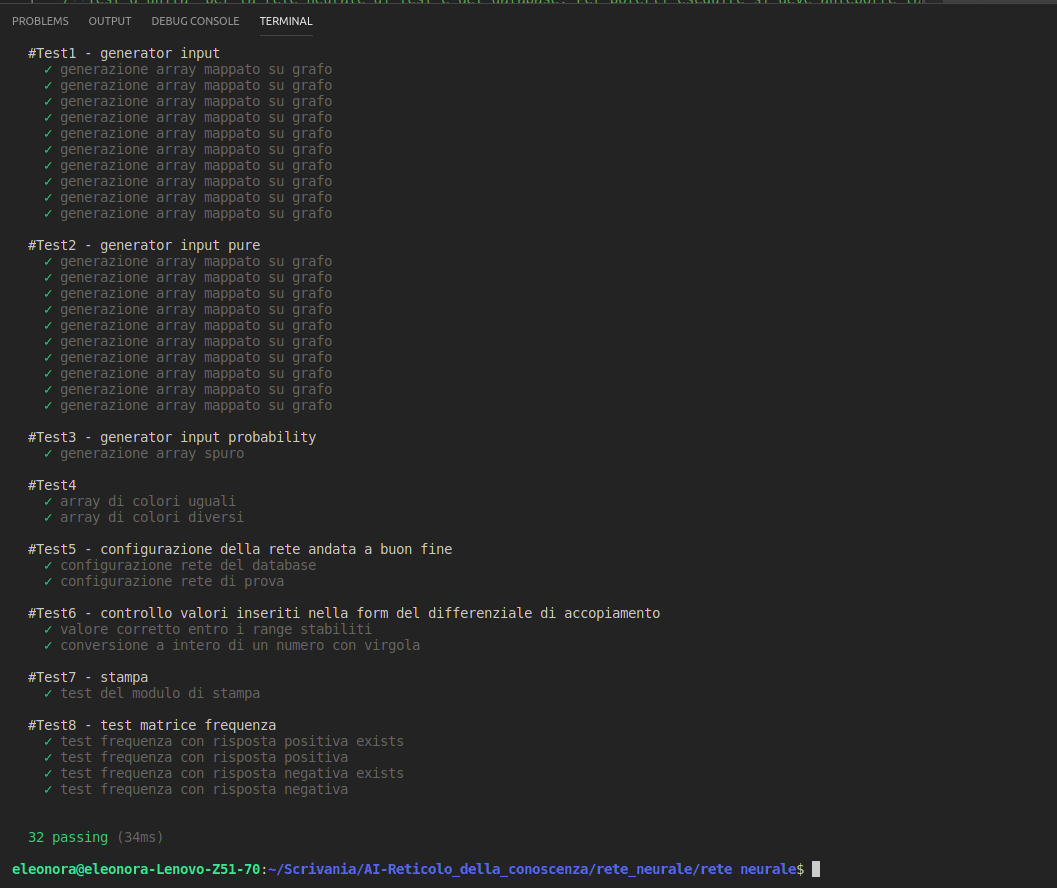
\includegraphics[width=0.80\linewidth]{./image/recap_test.png}
	\caption{Resoconto unit test con successo.}
	\label{Resoconto unit test con successo.}
\end{figure}
\noindent

\subsection{Sistema operativo e browser}
Il progetto \`e stato sviluppato su sistema operativo Linux e testato sul sistema operativo Windows, messo a disposizione in ufficio. L'applicativo della Rete neurale \`e sviluppato ad hoc per browser Chrome in cui il caricamento di grandi moli di dati ha nettamente prestazioni migliori. Sconsiglio l'utilizzo dell'applicativo sviluppato su Microsoft Edge e Firefox , in quanto il caricamento del file di allenamento \`e molto lento \footnote{se il file ha dimensioni superiore a 1000 entry.}.

\subsubsection{Specifiche di sviluppo}
\label{Specifiche di sviluppo}
\begin{itemize}
\item Sistemi operativi di sviluppo:
\begin{itemize}
\item Versione sistema operativo di sviluppo principale: Ubuntu 4.15.0-52.56-generic 4.15.18;
\item Versione sistema operativo pc fisso aziendale: Windows 10 Enterprise, versione 1809;
\end{itemize}
\item Browser di testing:
\begin{itemize}
\item browser principale: Chrome versione 75.0.3770.100 a 64 bit e Versione 66.0.3359.170 a 64 bit;
\item browser (sconsigliato per l'uso della Rete del database): Microsoft Edge 44.17763.1.0, Microsoft EdgeHTML 18.17763;
\item browser (sconsigliato per l'uso della Rete del database): Firefox Quantum 67.0.2 a 64 bit.
\end{itemize}
\item Strumenti di codifica:
\begin{itemize}
\item Visual Studio Code 1.35.1.
\end{itemize}
\item Strumenti di documentazione:
\begin{itemize}
\item Texmaker 5.0.3 (compiled with Qt 5.9.5).
\end{itemize}
\end{itemize}
\noindent
Il progetto \`e mantenuto all'interno di una piattaforma pubblica, con directory anch'essa pubblica. Sia il codice implementato che la documentazione sono soggetti a controllo di versione.  L'indirizzo http dove la directory \` e posizionata, \`e il seguente:
\begin{center}\url{https://github.com/esignor/AI-Reticolo_della_conoscenza}\end{center}.